\definecolor{bblue}{HTML}{0064FF}
\definecolor{rred}{HTML}{C0504D}
\definecolor{ggreen}{HTML}{9BBB59}
\definecolor{ppurple}{HTML}{9F4C7C}

\definecolor{b1}{HTML}{BEE9E8}
\definecolor{b2}{HTML}{188FA7}

\begin{figure}[!t]
\centering
\scalebox{0.85}{
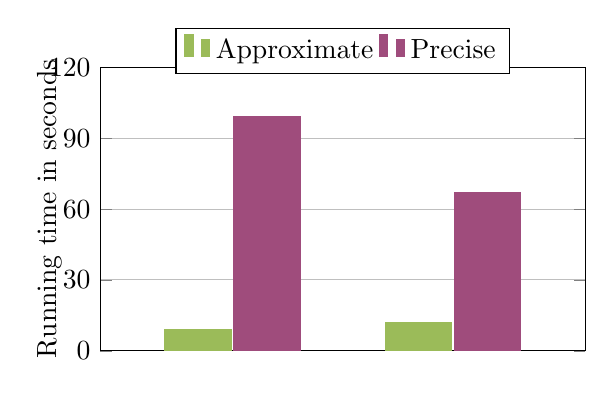
\begin{tikzpicture}
    \begin{axis}[
        width  = 8cm,
        height = 8cm,
        y=0.03cm,
        x=2.8cm,
        major x tick style = transparent,
        ybar=2*\pgflinewidth,
        bar width=24pt,
        ymajorgrids = true,
        ylabel = {Running time in seconds},
        ylabel style={yshift=-4mm},
        symbolic x coords={\batchoverflow,\reentrancy},
        ytick={0,30,60,90,120},
        xtick = data,
        scaled y ticks = false,
        enlarge x limits=0.6,
        ymin=0,
        ymax=120,
        legend cell align=left,
        legend entries={Approximate, Precise},
        legend style={
                at={(0.5,1.14)},
                legend columns=-1,
                anchor=north,
        %        column sep=1ex
        }
    ]
    %\hspace*{-2mm}
        \addplot[style={ggreen,fill=ggreen,mark=none}]
        coordinates{(\batchoverflow,9)(\reentrancy,12)};

        \addplot[style={ppurple,fill=ppurple,mark=none}]
        coordinates{(\batchoverflow,99)(\reentrancy,67)};
    \end{axis}
\end{tikzpicture}
}
% \vspace{-0.2in}
\caption{Average running time under different settings}
\vspace{-0.2in}
\label{fig:eval-oyente}
\end{figure}
